% 02.06.2016 12:00 CET last changed by a.holzinger
% General Template for LNCS and LNAI contributions based on llncs, adapted by ah
% Many thanks to the TRS team
% In case of using eps compile via 1) TeXify and then proceed with 2) dvi2pdf
%
\documentclass{llncs}
\usepackage{float}

\usepackage[dvips]{graphicx}
\usepackage[ruled,vlined]{algorithm2e}
\usepackage{amsfonts}
\usepackage{amssymb}
\usepackage{amsmath}
\usepackage{mathtools}

\providecommand{\abs}[1]{\lvert#1\rvert}
\providecommand{\norm}[1]{\lVert#1\rVert}

\usepackage{calc}
\usepackage{subfigure}

\usepackage{color}
\usepackage{soul}
\usepackage{comment}

\newtheorem{prop}{Property}

\newenvironment{Bitemize}{\renewcommand\labelitemi{\textbullet}\begin{itemize}}{\end{itemize}}

\begin{document}

\title{DO NOT DISTURB ? \\ Classifier behavior on perturbed datasets}

% \author{Bernd Malle\inst{1}\inst{2}, Peter Kieseberg\inst{1}\inst{2}, Edgar Weippl\inst{2}, Andreas Holzinger\inst{1}}

%\institute{Holzinger Group HCI-KDD \\
%Institute for Medical Informatics, Statistics \& Documentation\\
%            Medical University Graz, Austria\\
%            \texttt{b.malle@hci-kdd.org}
%\and
%SBA Research gGmbH, Favoritenstraße 16, 1040 Wien \\
%			\texttt{PKieseberg@sba-research.org}
%}
	
\maketitle

% ==================================
%				ABSTRACT
% ==================================
\begin{abstract}

Exponential trends in data generation are presenting todays organizations, economies and governments with challenges never encountered before, especially in the field of privacy and data security. One crucial trade-off regulators are facing regards the simultaneous need for publishing personal information for the sake of statistical analysis and Machine Learning in order to increase quality levels in areas like medical services, while at the same time protecting the identity of individuals. A key European measure will be the introduction of the General Data Protection Regulations (GDPR) in 2018, giving customers the 'right to be forgotten', i.e. having their data deleted on request. As this could lead to a competitive disadvantage for European companies, it is important to understand which effects deletion of significant data points has on the performance of ML techniques. In a previous paper we introduced a series of experiments applying different algorithms to a binary classification problem under anonymization as well as perturbation. In this paper we extend those experiments by multi-class classification and introduce outlier-removal as an additional scenario. While the results of our previous work were mostly in-line with our expectations, our current experiments revealed unexpected behavior over a range of different scenarios.


\medskip

\textbf{Keywords}: Machine learning, knowledge bases, right to be forgotten, perturbation, k-anonymity, SaNGreeA, information loss, cost weighing vector, multi-class classification, outlier analysis, variance-sensitive analysis


\end{abstract}

\renewcommand{\thesubfigure}{\thefigure.\arabic{subfigure}}
\makeatletter
\renewcommand{\p@subfigure}{}
\renewcommand{\@thesubfigure}{\thesubfigure:\hskip\subfiglabelskip}
\makeatother


% ==================================
%			INTRODCUTION
% ==================================
\section{Introduction and Motivation for Research}


% ==================================
%			RELATED WORK
% ==================================

A comparison of different Machine Learning algorithms on anonymized datasets was already conducted in 2014 (\cite{Wimmer2014}) by applying 6 different algorithms on 3 datasets, with very diverse results per algorithm. The main weakness of this paper is its usage of extremely differently-sized datasets which does not easily allow comparison; moreover they only used one very low privacy setting of $k=2$, preventing the authors from examining more interesting behavior as information content degrades further; this is a main point of our work.

\cite{Majeed2017}



% ==================================
%			BASICS K-ANONYMITY
% ==================================
\section{Scenarios of incurring information loss in datasets}


\subsection{Tabular anonymization}
\label{ssect:tab_anonym}

% Figure~\ref{fig:anon_categories} illustrates the original tabular concept of anonymization: Given an input table with several columns, we will in all probability encounter three different categories of data:

% \begin{itemize}
%	\item \textbf{Personal identifiers} are data items which directly identify a person without having to cross-reference or further analyze them. Examples are first and last names, but even more so an (email) address or social security number (SSN). As personal identifiers are dangerous and cannot be generalized (see Figure~\ref{fig:gen_hierarchy}) in a meaningful way (e.g. one could generalize an email address by only retaining the mail provider fragment, but the result would not yield much usable information), this category of data is usually removed. The table shows this column in a red background color.
%	\item \textbf{Sensitive data,} also called 'payload', which is the kind of data we want to convey for statistics or research purposes. Examples for this category would be disease classification, drug intake or personal income level. This data shall be preserved in the anonymized dataset and can therefore not be deleted or generalized. The table shows this column in a green background color.
%	\item \textbf{Quasi identifiers (QI's)}, colored in the table with an orange background, are data that in themselves do not directly reveal the identity of a person, but might be used in aggregate to reconstruct it. For instance, \cite{sweeney2002k} mentioned that 87\% of U.S. citizens in 2002 had reported characteristics that made them vulnerable to identification based on just the 3 attributes \textit{zip code}, \textit{gender} and \textit{date of birth}. But although this data can be harmful in that respect, it might also hold vital information for the purpose of research (e.g. zip code could be of high value in a study on disease spread). The the actual point of all anonymization efforts is therefore to generalize this kind of information, which means to lower its level of granularity. As an example, one could generalize the ZIP codes 41074, 41075 and 41099 to an umbrella version 410**, as shown in Figure~\ref{fig:anonymized_clusters}.
%\end{itemize}

\begin{figure}[!t]
	\begin{center}
		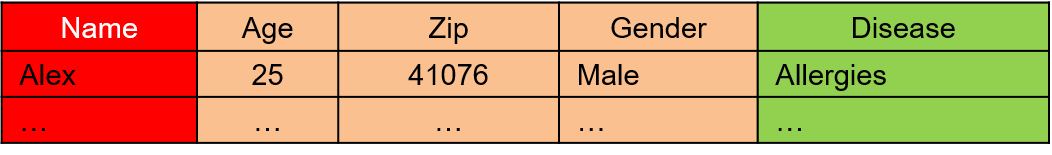
\includegraphics[width=\textwidth]{figures/theory/3typesofdata}
		\caption{The three types of data considered in (k-)anonymization}
		\label{fig:anon_categories}
	\end{center}
\end{figure}

%As described in \cite{ciriani2007kappa}, k-anonymization requires that in each data release every combination of values of quasi-identifiers must be identical to at least $k-1$ other entries in that release, which can be seen as a clustering problem with each cluster's (also called \textit{equivalence class}) quasi-identifier state being identical for every data point. This can be achieved via suppression and generalization, where suppression means simply deletion, whereas in generalization we try to retain some usable value.

%The process of generalization works through a concept called \textit{generalization hierarchies}, which form a tree, whose root denotes the most general value available for an attribute (usually the 'all' value) and then branches to more and more specific occurrences, with its leafs representing the set of exact, original values (see Figure~\ref{fig:gen_hierarchy}). In generalizing the original input value, one traverses the tree from the leaf level upwards until a prerequisite is fulfilled. Usually, this comes in the form of the k-anonymity requirement, so that we want to find a group of other data entries whose generalized QI's match the data point being processed.

\begin{figure}[!t]
	\begin{center}
		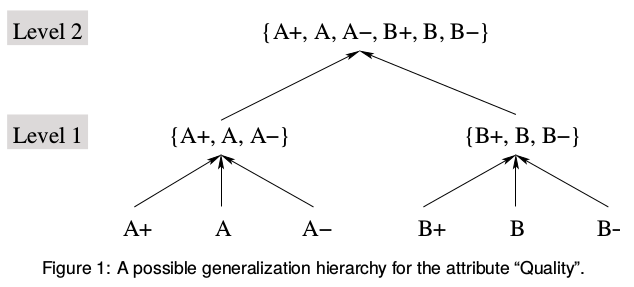
\includegraphics[width=\textwidth]{figures/theory/gen_hierarchy}
		\caption{Example of a typical generalization hierarchy}
		\label{fig:gen_hierarchy}
		\small
		taken from \cite{aggarwal2005approximation}
	\end{center}
\end{figure}


%Each level of generalization involves a certain cost in information loss, so we do not want to construct our clusters in any random sequence but minimize the overall information loss \cite{aggarwal2005approximation}. This makes k-anonymization an NP-hard problem due to an exponential number of possible generalized QI combinations.

\begin{figure}[!t]
	\centering
	\begin{minipage}[b]{0.535\textwidth}
		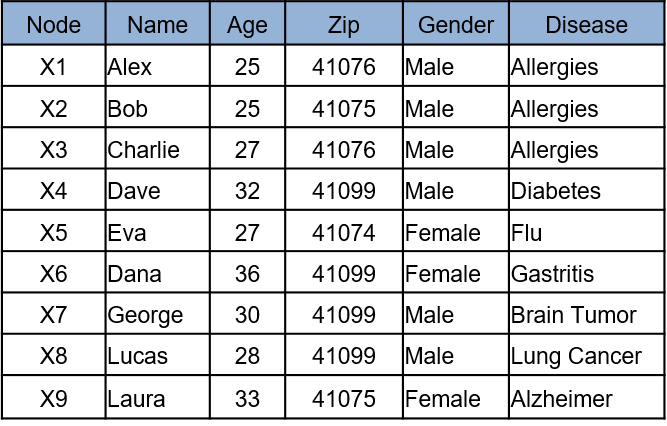
\includegraphics[width=\textwidth]{figures/theory/k_anon_input}
	\end{minipage}
	\hfill
	\begin{minipage}[b]{0.448\textwidth}
		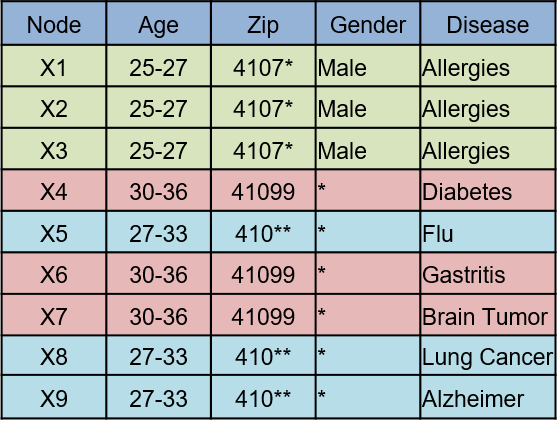
\includegraphics[width=\textwidth]{figures/theory/k_anon_output}
	\end{minipage}
	\caption{Tabular anonymization: input table and anonymization result}
	\label{fig:anonymized_clusters}
\end{figure}



% ==================================
%				EXPERIMENTS
% ==================================
\section{Experiments}
\label{sect:experiments}

The following sections will describe our series of experiments in detail, encompassing the data source selected, the algorithm used as well as a description of the overall process employed to obtain our results.


\subsection{Data} 
\label{ssect:data}

As input data we chose the adults dataset from the UCI Machine Learning repository which was generated from US census data of 1994 and contains approximately 32,000 entries; from those 30,162 were selected after preprocessing. Of the attributes (data columns) provided only one was deleted because it was also represented by a column containing its numerical mapping (education $=>$ education\_num). Figure~\ref{fig:adult_original_distribution} shows the attribute value distribution of the original input dataset with the exception of the sample weights.


\begin{figure}[!t]
	\begin{center}
    \hspace*{-0.8cm}
		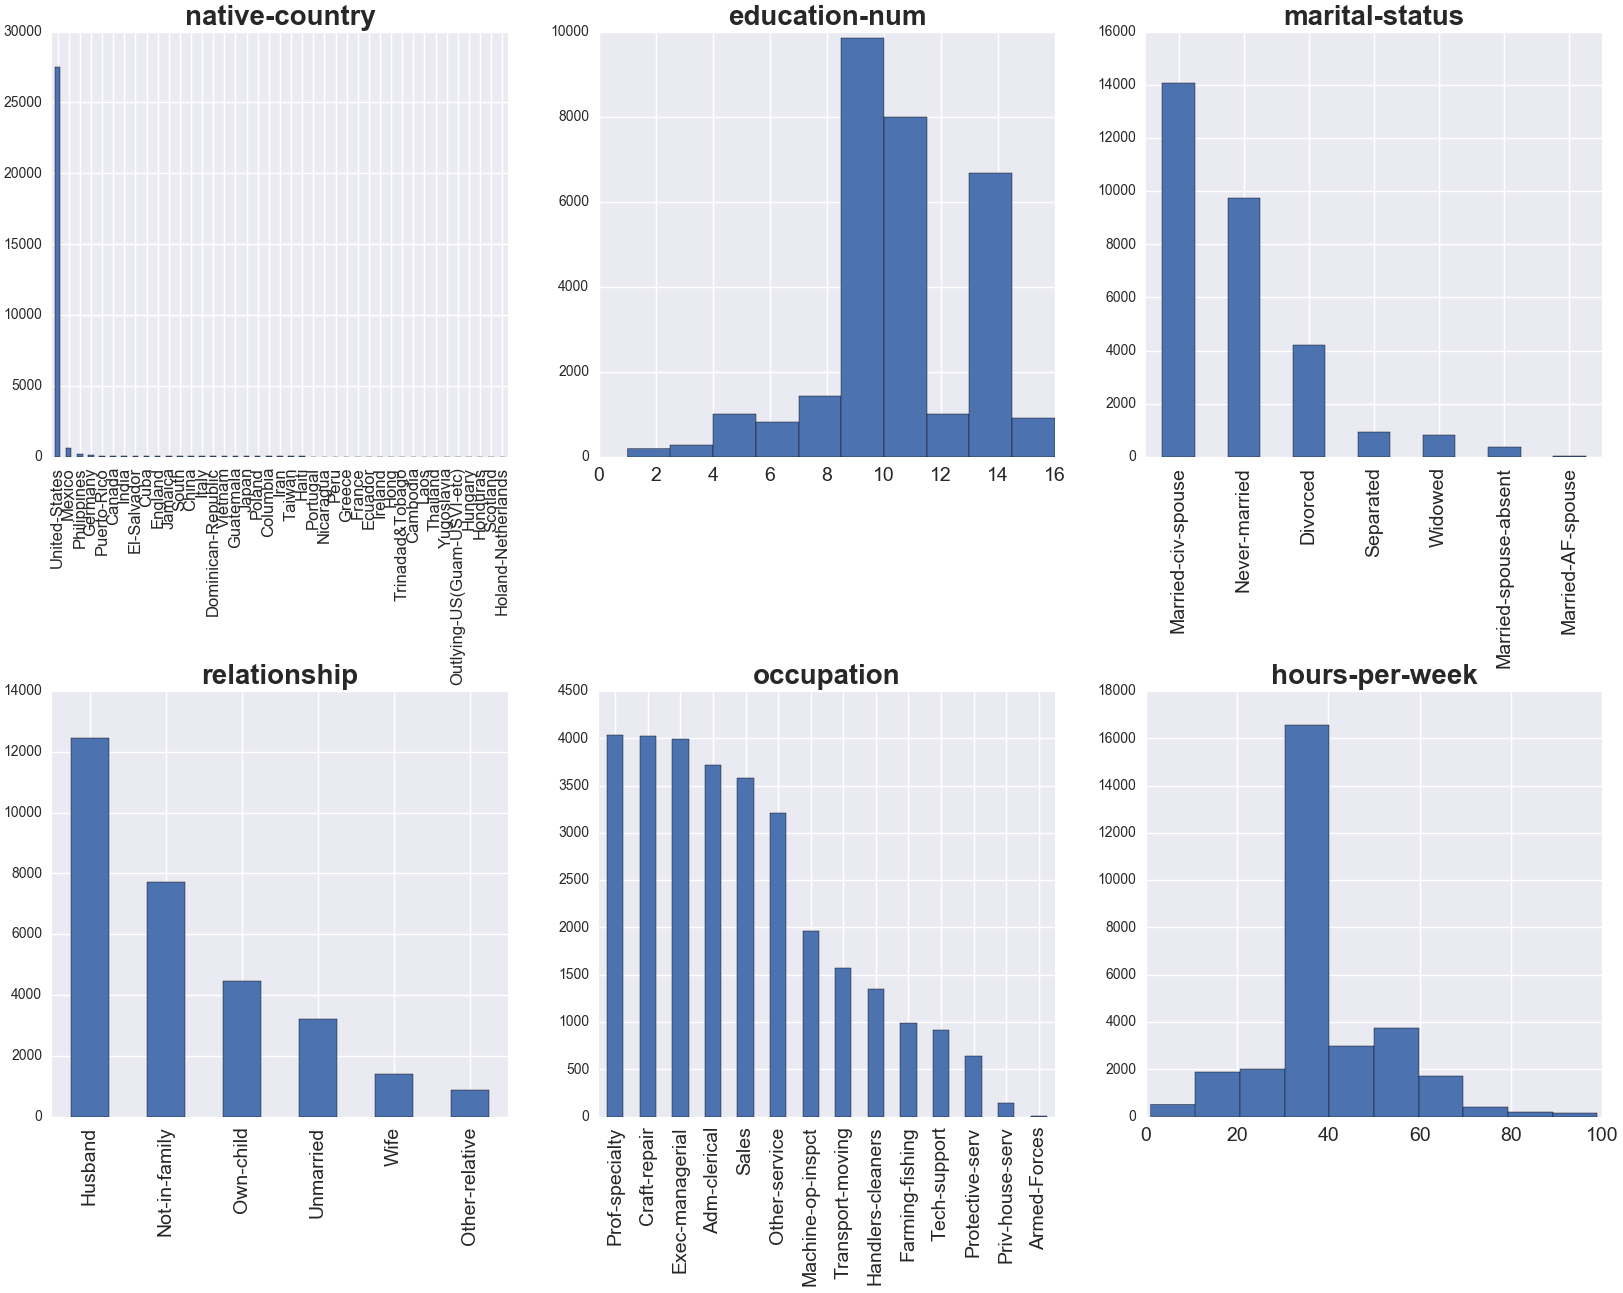
\includegraphics[width=1.1\textwidth]{figures/theory/dist_initial_small}
		\caption{Initial distribution of six selected data columns of the adult dataset.}
		\label{fig:adult_original_distribution}
	\end{center}
\end{figure}

% As one can see, there are several attributes with one value clearly dominating the others; \textit{native-country} being the most prominent example with the entry for the United States dwarfing all other countries (which comes as no surprise given the data origin). As anonymization generalizes different countries together if necessary, it was interesting for the author to see how these distributions would change under a relatively large k-factor. Figure~\ref{fig:adult_anonymized_distribution} shows the same attribute distribution with its values anonymized by a factor of $k=19$. Although the dominance of the United states was successfully "broken" by this method, in several instances the \textit{generalized-to-all}-value (*) now skews the data set even more. Apart from the expected generalization information loss this is another reason why one would assume worse results from a machine learning classifier applied to an anonymized dataset.

\begin{figure}[!t]
	\begin{center}
    	\hspace*{-0.8cm}
		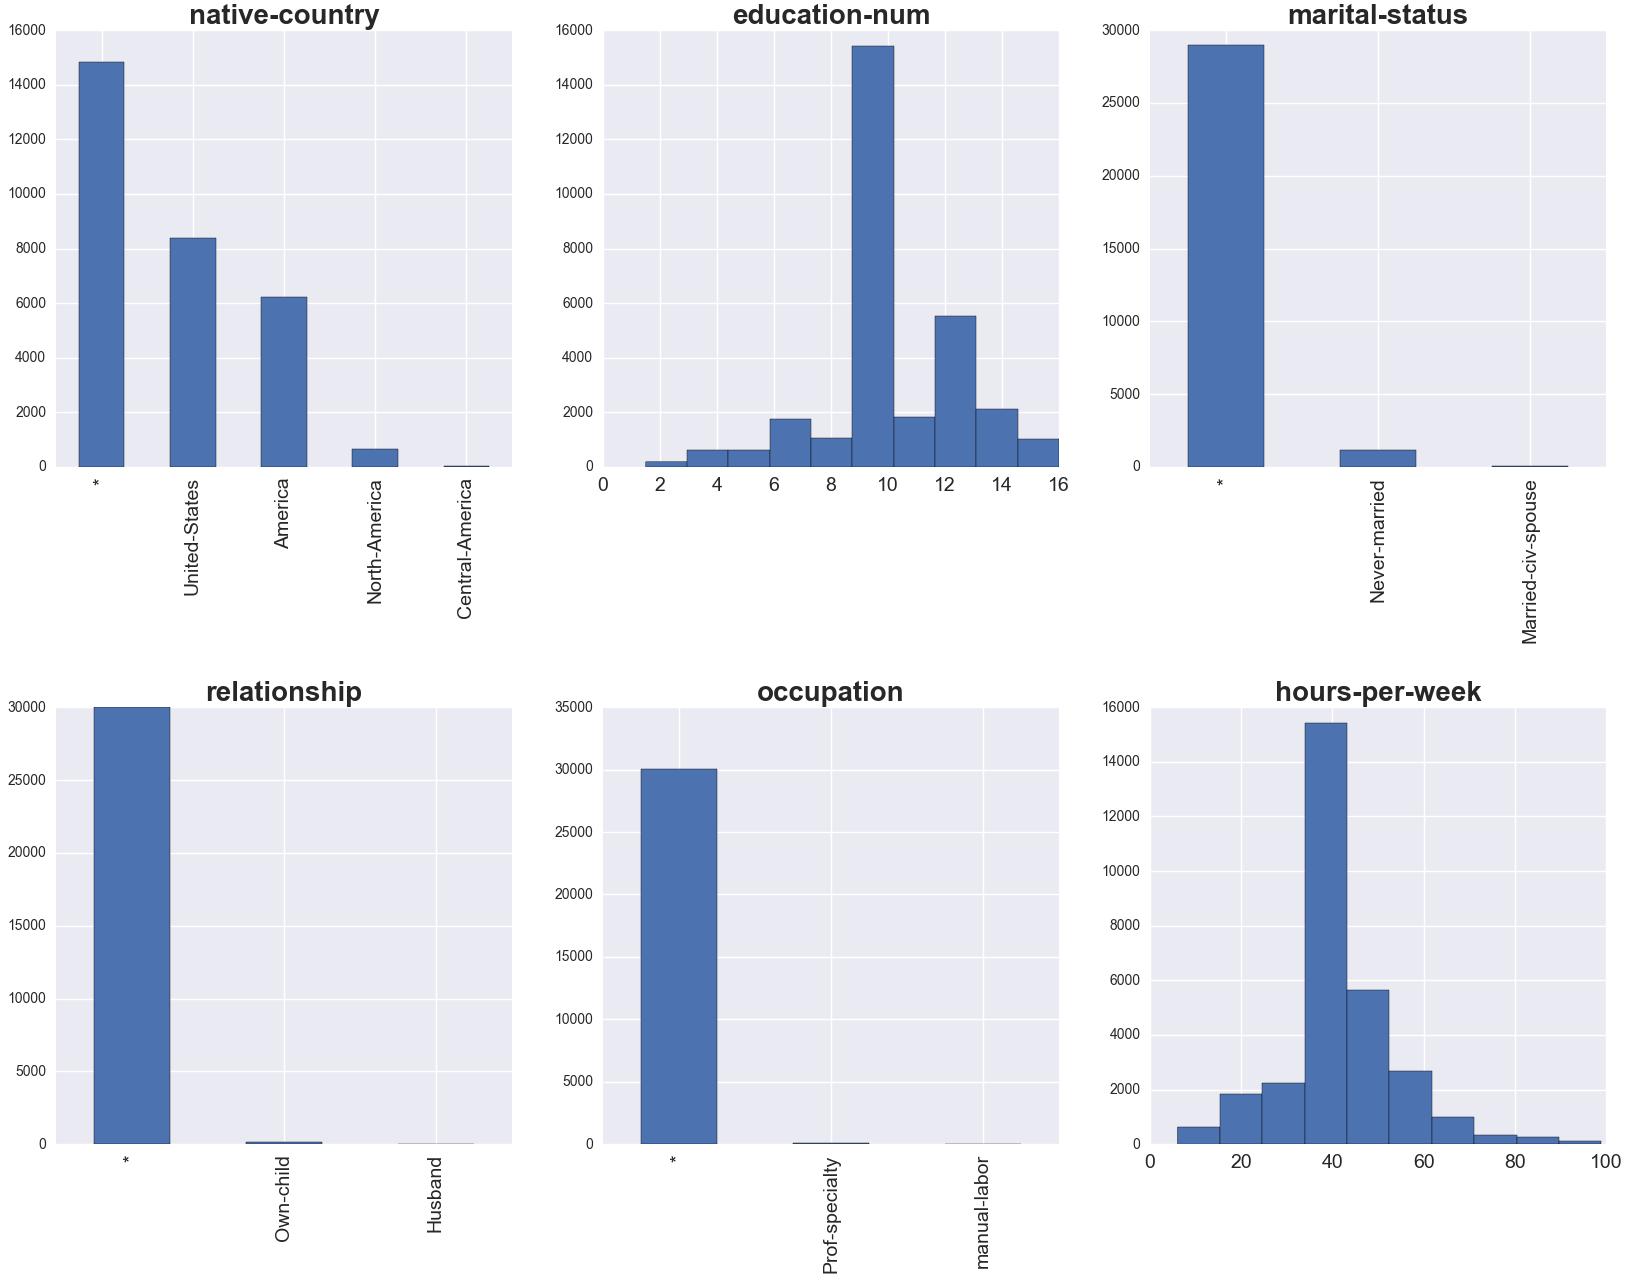
\includegraphics[width=1.1\textwidth]{figures/theory/dist_anonym_small}
		\caption{Anonymized distribution of six selected data columns of the adult dataset, anonymization factor of k=19, equal weight for each attribute.}
		\label{fig:adult_anonymized_distribution}
	\end{center}
\end{figure}



\subsection{Algorithm}
\label{ssect:algorithm}

% SaNGreeA stands for \textit{Social network greedy clustering} and was introduced by \cite{campan2009data}. In addition to 'clustering' nodes of a graph according to the minimum general information loss (GIL) incurred as described in Section~\ref{ssect:tab_anonym}, this algorithm also considers the structural information loss (SIL) incurred in assigning a node to a certain cluster. The SIL quantifies the probability of error when trying to reconstruct the structure of the initial graph from its anonymized version.

\begin{equation*}
\begin{split}
\text{GIL}(cl) = \abs{cl} \cdot (\sum_{j=1}^{s} \frac{size(gen(cl)[N_j])}{size(min_{x \epsilon N} (X[N_j]), max_{x \epsilon N} (X[N_j]))} \\ 
+ \sum_{j=1}^{t} \frac{height(\Lambda(gen(cl)[C_j]))}{height(H_{C_j})})    
\end{split}    
\end{equation*}


where:\\
- $\abs{cl}$ denotes the cluster cl's cardinality; \\
- $size([i1,i2])$ is the size of the interval $[i1,i2]$, i.e., $(i2-i1)$; \\
- $\Lambda(w), w \epsilon H_{C_j}$ is the sub-hierarchy of $H_{C_j}$ rooted in $w$; \\
- $height(H_{C_j})$ denotes the height of the tree hierarchy $H_{C_j}$; \\


The total generalization information loss is then given by:
\begin{equation*}
\text{GIL}(G,S) = \sum_{j=1}^{v} \text{GIL}(cl_j)
\end{equation*}
And the normalized generalization information loss by:
\begin{equation*}
\text{NGIL}(G,S) = \frac{\text{GIL}(G,S)}{n \cdot (s+t)}
\end{equation*}

% The SIL is composed of two different components: 1) the intra-cluster structural loss, signifying the error probability in trying to reconstruct the original edge distribution within an equivalence class (= anonymized cluster), and 2) the inter-cluster structural loss which represents the error probability in trying to reconstruct the original configuration of edges between two equivalence classes.

% For the exact mathematical definitions of SIL \& NSIL the reader is kindly referred to the original paper. Because the structural information loss cannot be computed exactly before the final construction of clusters, the exact computations were replaced by the following distance measures: \\

Distance between two nodes:
\begin{equation*}
\text{dist}(X^i, X^j) = \frac{\abs{\{l|l=1..n \wedge l \ne i,j;b_l^i \ne b_l^j}}{n-2}
\end{equation*}

Distance between a node and a cluster:
\begin{equation*}
\text{dist}(X, cl) = \frac{\sum_{X^j \epsilon cl} \text{dist}(X, X^j) }{\abs{cl}}
\end{equation*}


% The algorithm starts with initializing a first cluster by a randomly choosing a node. Then, for every new node encountered, the weighted sum of the above two information loss metrics will yield a certain overall information loss in case the node was added to that cluster - the candidate with minimal information loss is then added to the cluster. This process is repeated until the cluster reaches a certain constraint (e.g. size $ \coloneqq  k $ -factor) upon which another random node is chosen to constitute the next cluster. This procedure is repeated until all nodes have been assigned; if a cluster of size $< k$ should remain, its member nodes are dispersed accordingly.

% Since the algorithm does not take all possible node combinations into account, but simply chooses an arbitrary node and compares all the candidates in a loop, the algorithm runs in quadratic time w.r.t. the input size in number of nodes. This worked well within milliseconds for a problem size of a few hundred nodes, but took up to 60 mins. on the whole adult dataset.

% In implementing and demonstrating this algorithm, the authors intended to recreate the original paper's experiment. However, as no suitable real-world graph structure was available to the authors at the time of this writing and any artificially generated network would result in dubious results for the classification tasks applied, we decided to leave out the structural component of the algorithm and focus only on the generalization information loss for this paper, leaving the entire approach to future research initiatives.



\subsection{Process}
\label{ssect:process}

To examine the effect of perturbation and anonymization on classification performance, we designed the following processing pipeline:


%\begin{enumerate}
%	\item Taking the original (preprocessed) dataset as input, we transformed its attributes to boolean values, so instead of \textit{native-country $->$ United-States} we considered \textit{United-States $->$ yes / no}.
%	\item We then ran 4 different classifiers on it and computed precision, recall as well as F1 score. The four classifiers used were \textit{gradient boosting}, \textit{random forest}, \textit{logistic regression} and \textit{linear SVC}.
%	\item From the obtained results we extracted the 3 attribute values most contributing to a "positive" ($>$50k) result as well as the top 3 attribute values indicating a "negative" ($<=$50k) prediction as depicted in Figure~\ref{fig:adult_important_columns}
%	\item For each of these 6 attribute values, we subsequently deleted a specific percentage of data rows containing that value from the original dataset, resulting in 30 reduced datasets. The 5 percentages used were $0.2$, $0.4$, $0.6$, $0.8$ as well as $1.0$.
%	\item To each of those datasets we re-applied the four chosen classifiers successively and recorded the respective impact on the quality of the classification result. The results can be seen in Figure~\ref{fig:adult_results_perturbation_top} and Figure~\ref{fig:adult_results_perturbation_bottom}.
%	\item In order to measure the effects of k-anonymization on classifier performance, we used the SaNGreeA's GIL component described in the following section to generate datasets with a k-factor of $k=3$, $k=7$, $k=11$, $k=15$ as well as $k=19$. Furthermore, we used each of these settings with 3 different weight vectors: 1) equal weights for all attributes, 2) age information preferred ($\omega(age)=0.88$, $\omega(other\_attributes)=0.01$) and 3) race information preferred ($\omega(race)=0.88$, $\omega(other\_attributes)=0.01$). We then re-executed all classifiers on the resulting 15 datasets and recorded the respective results, which can be seen in Figure~\ref{fig:adult_results_anonymization}.
%\end{enumerate}


\begin{figure}[!h]
	\begin{center}
		% \vspace{-1.0cm}
    	\hspace*{-0.8cm}
		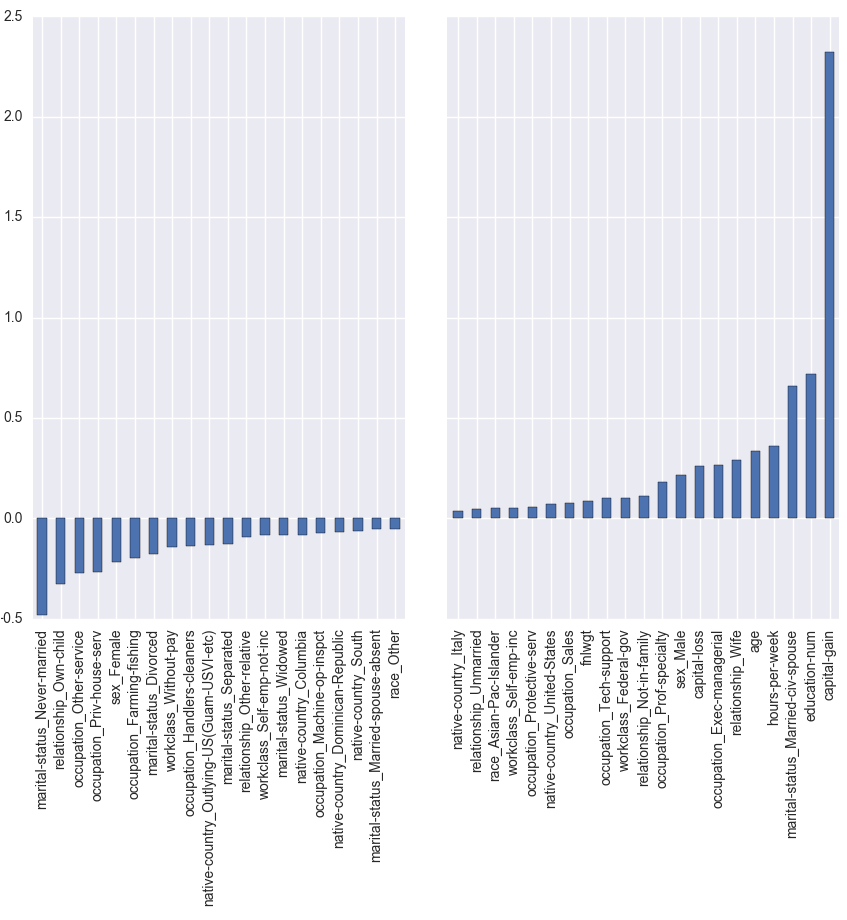
\includegraphics[width=1.1\textwidth]{figures/theory/important_columns_cut}
		\caption{Attribute values within the adult dataset which contribute highest / lowest certainty to the classification result. The rightmost columns represent information which enable a classifier to discern most clearly between classes, while the leftmost columns (depending on their actual score) could even confuse the algorithm. }
		\label{fig:adult_important_columns}
	\end{center}
\end{figure}


% ==================================
%		RESULTS & DISCUSSION
% ==================================
\section{Results \& Discussion}
\label{sect:results}


\subsection{Perturbed Datasets - Selective Deletion}
\label{ssect:selective_deletion}

In order to be able to compare the impact of selectively deleting the most / least important attribute values (in fact, the whole data points containing those values) on different classifiers, we chose to select these values via examining the logit coefficients from logistic regression. Although this possibly entails non-erasure of the values specifically significant for each classifier, we chose algorithmic comparison as the more insightful criterion; the implicit assumption that the same attribute values would influence all classifiers approximately equally was largely confirmed by our results.

In contrast to binary classification, determining the 'right' values to delete for a multi-class problem is not always possible: Values contributing highly to the decision boundary for one class might be less significant in the case of another - accordingly one would expect inconclusive behavior in the case of a target for which the highest / lowest log coefficients do not line up over class boundaries.

For each of the targets 'marital-status' and 'education-num' we measured those interesting coefficients in the hope of improving / degrading algorithmic performance; that means deletion of highest logit's is supposed to remove certainty from an algorithm and decreasing performance, while deletion of lowest logit's is supposed to remove uncertainty, thus improving performance. Our analysis showed that while 'marital-status' had mainly the same most / least significant logit's across all classes, the attribute values for 'education-num' were rather diverse in this area.


In the latter case this lead to erratic behavior of the resulting performance curves, as can be seen in (Figure~\ref{fig:results_perturbation_education_num}). It is interesting to note that 'income$\_>$50k' obviously held much larger significance for Logistic Regression than for the other classifiers, as their results showed f1 score improvement with this particular value eviscerating.


\begin{figure*}[!h]
	\centering
	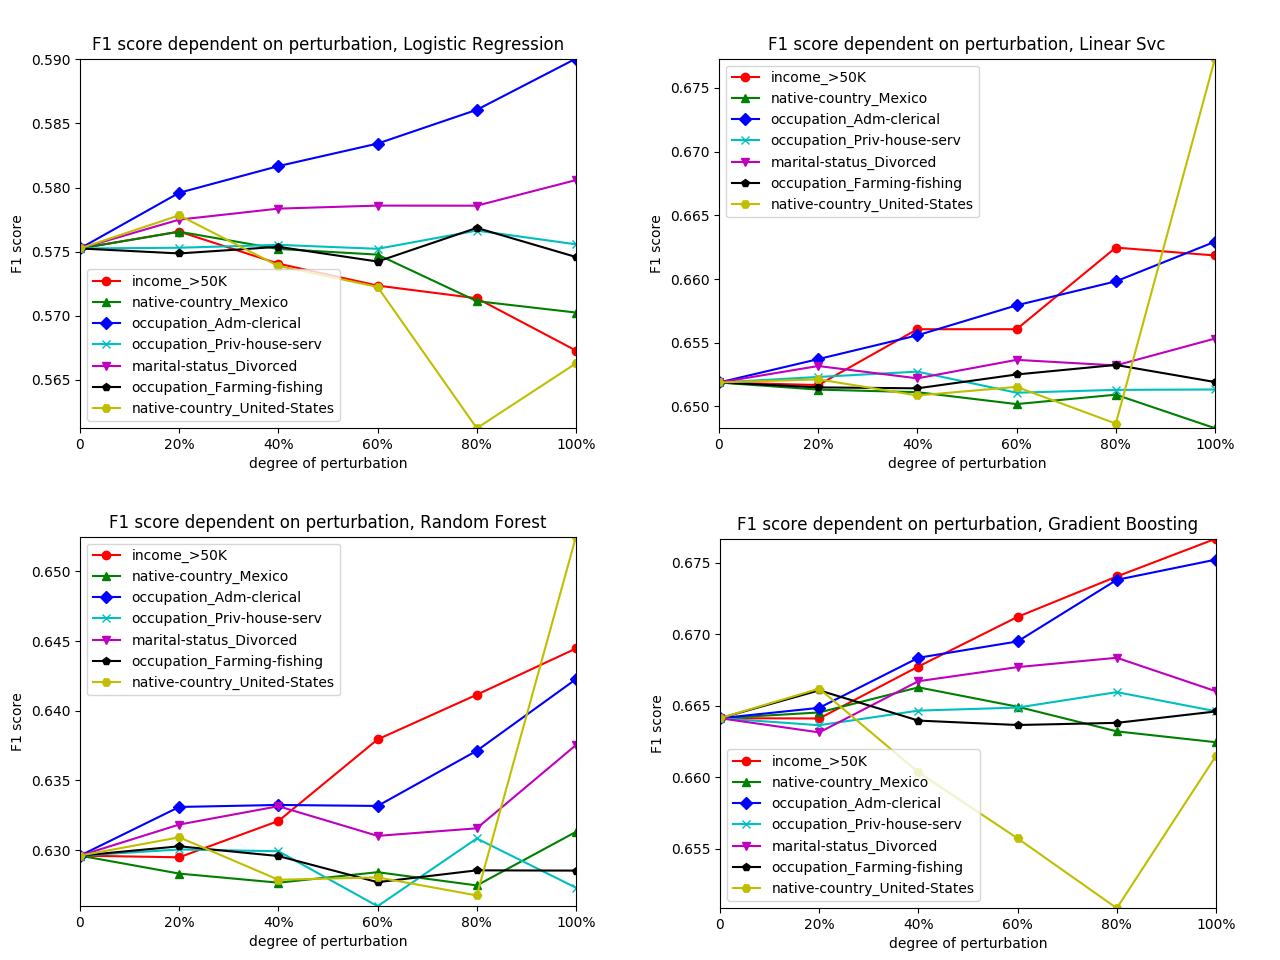
\includegraphics[width=1\textwidth]{figures/perturbation/adults_education_num/perturb_education_combined}
	\caption{Multi-class classification of 'education-num' under perturbation by selective deletion of the most (least) important data attributes.}
	\label{fig:results_perturbation_education_num}
\end{figure*}


In the case of 'marital-status' almost the same attribute values were rated as most / least significant across all classes - this results in very clear outputs with the erasure of highly important values decreasing performance drastically while deletion of confusing values leading to a significant increase in classifier performance (Figure~\ref{fig:results_perturbation_marital_status}). While it is not surprising that relationship information shows high correlation with marital status, the opposite effects of \textit{sex\_Female} and \textit{sex\_Male} stand out as a slight curiosity - being a woman in this dataset seems to point less distinctly to a specific marital status than being a man, seemingly at odds with a common sense view.


\begin{figure*}[!h]
	\centering
	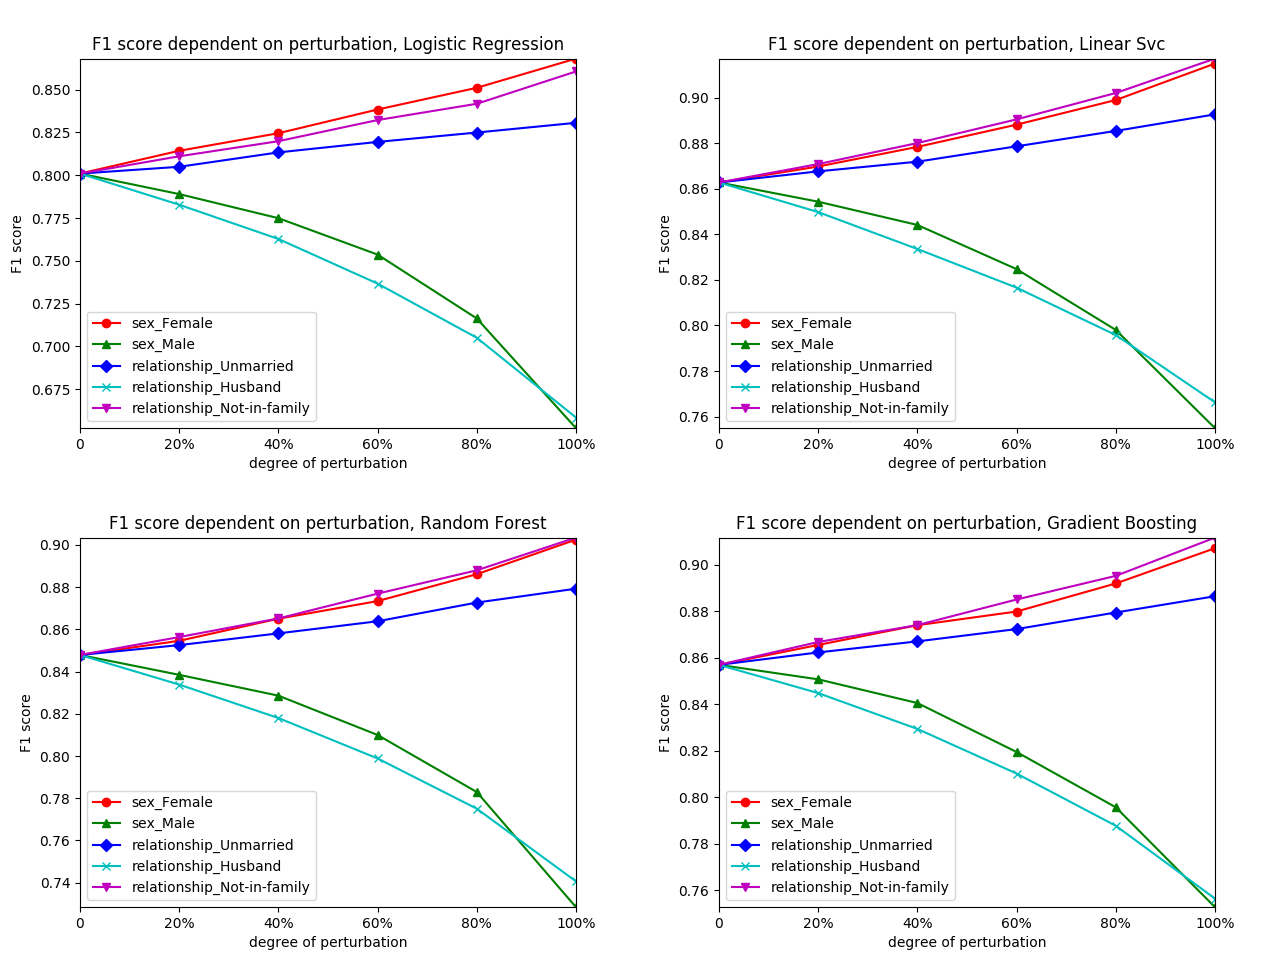
\includegraphics[width=1\textwidth]{figures/perturbation/adults_marital_status/perturb_marital_combined}
	\caption{Multi-class classification of 'marital-status' under perturbation by selective deletion of the most (least) important data attributes.}
	\label{fig:results_perturbation_marital_status}
\end{figure*}



\subsection{Anonymized Datasets}
\label{ssect:anonymized_ds}

% As far as the second case is concerned (Figure~\ref{fig:results_perturbation_marital_status}), our experiments showed the expected drop in algorithm performance, although the impact shows a different behavior: In the case of deleting rows with capital gain values of $>$ 2000 US-Dollars, the decline seems to be linear, whereas for the other two attribute values the performance seems to collapse with higher rates of erasure. Moreover, this behavior is more or less the same for all applied algorithms. This seems to point to the fact that especially significant attribute values can uphold a good performance even in low quantities.

\begin{figure*}[!h]
	\centering
	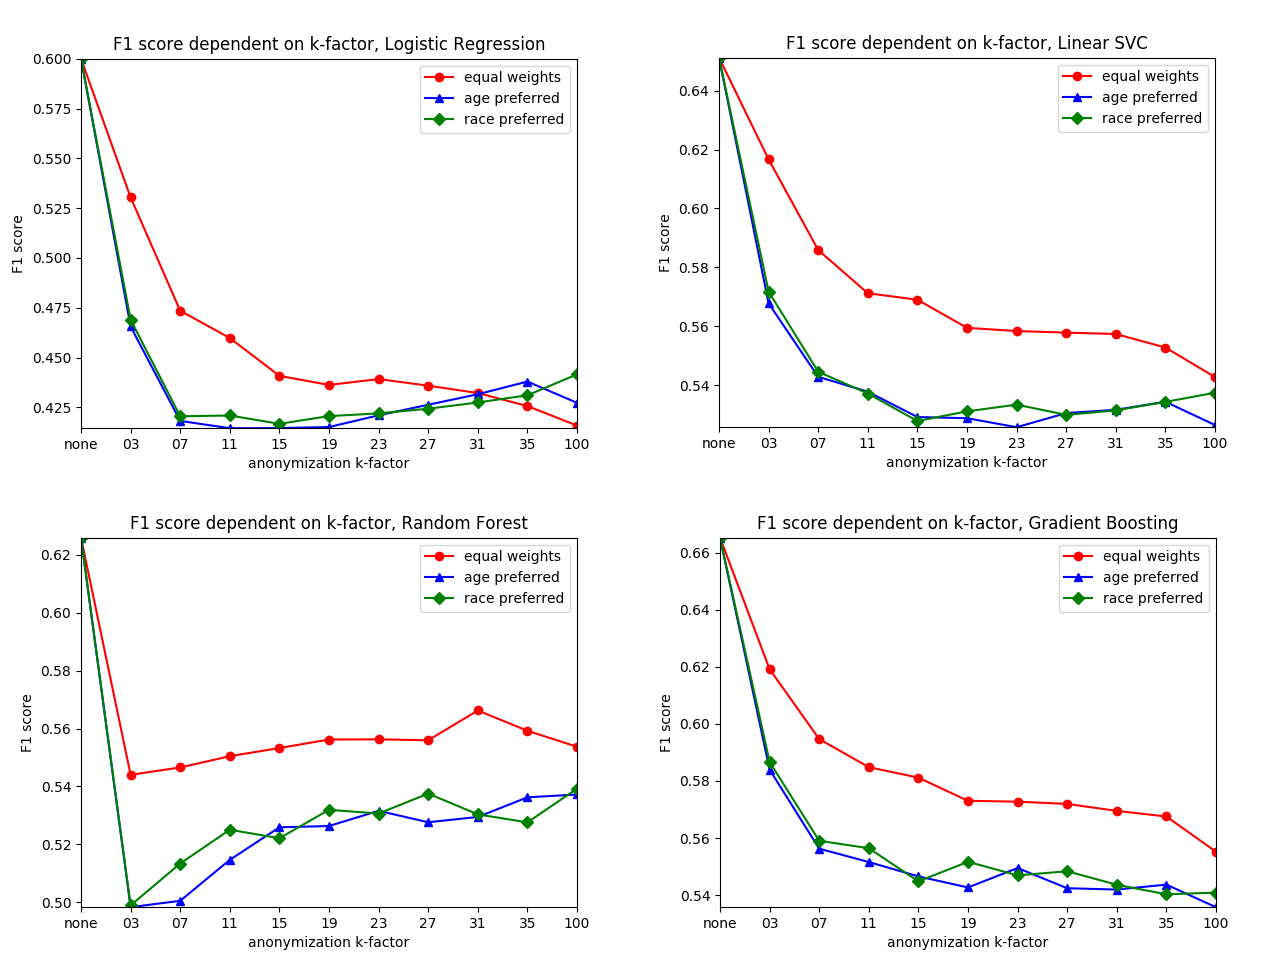
\includegraphics[width=1\textwidth]{figures/anonymization/adults_education_num/anon_education_combined}
	\caption{Multi-class classification of education num on the adult dataset under several degrees of k-anonymization.}
	\label{fig:results_anonymization_education_num}
\end{figure*}


\begin{figure*}[!h]
	\centering
	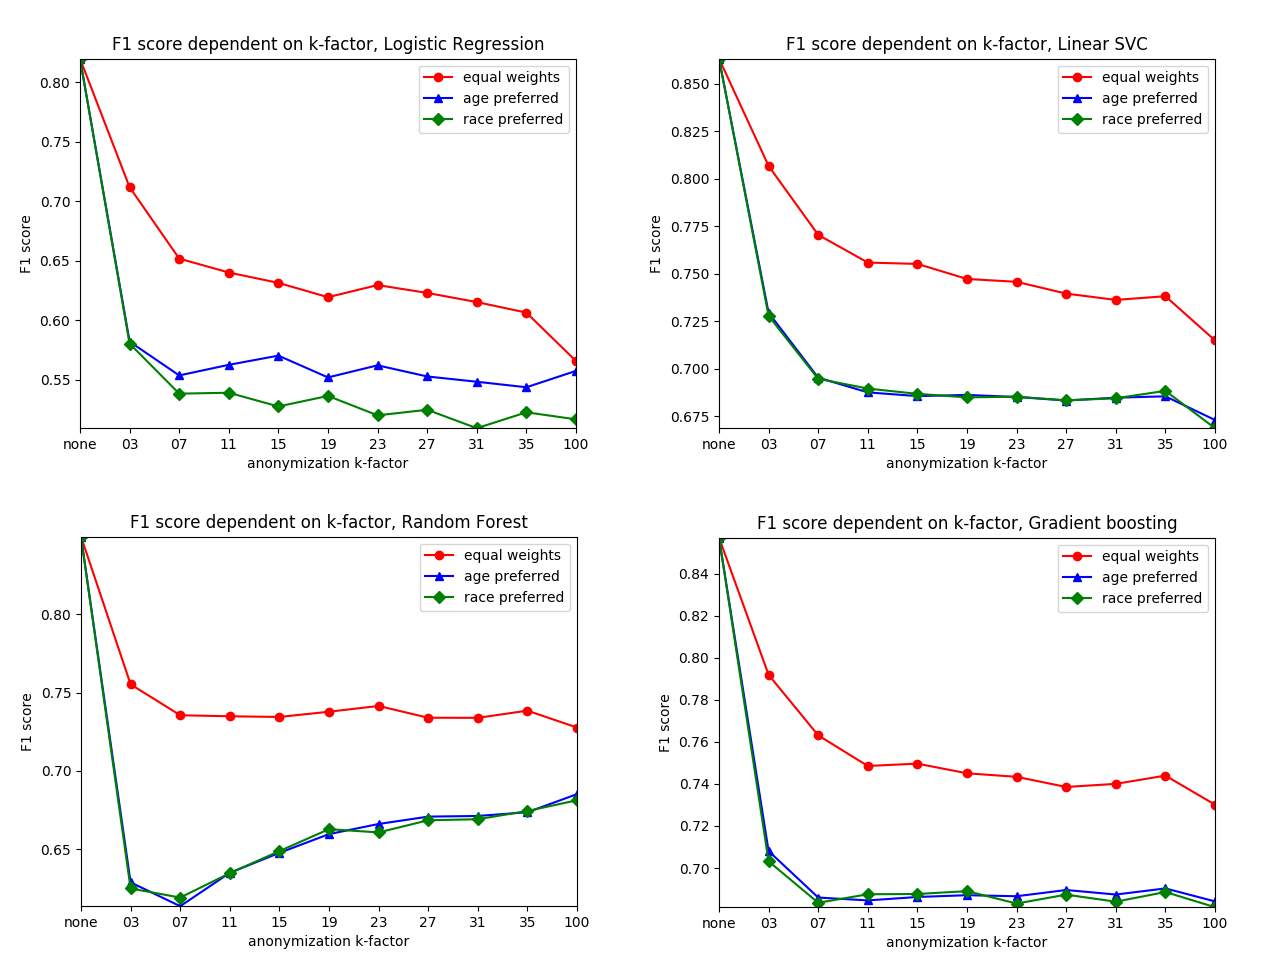
\includegraphics[width=1\textwidth]{figures/anonymization/adults_marital_status/anon_marital_combined}
	\caption{Multi-class classification of marital status on the adult dataset under several degrees of k-anonymization.}
	\label{fig:results_anonymization_marital_status}
\end{figure*}


% The only real surprise occurred with applying our classifiers to the datasets perturbed by deleting percentages of attribute values indicating a low yearly income (Figure~\ref{fig:adult_results_perturbation_bottom}). As with scenario 2 we expected to see a progressive decline in performance - but with all classifiers the results either stayed approximately the same or even improved in some cases (please consider the extremely narrow scale in the respective plots). As the classification score is dependent on (in-)correctly classifying both positive and negative outcomes, this seems rather surprising and will require further investigation.


\subsection{Outliers removed}
\label{ssect:outliers_removed}

\begin{figure*}[!h]
	\centering
	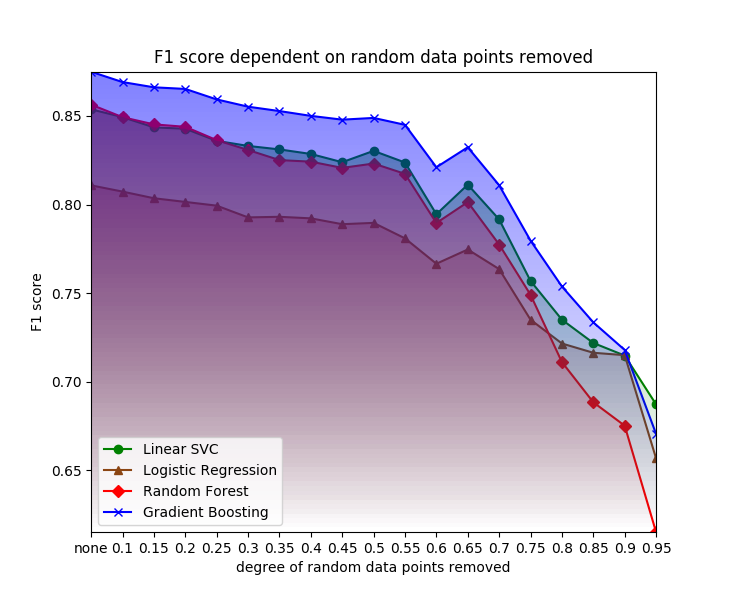
\includegraphics[width=0.49\textwidth]{figures/outliers/outliers_removed_all_algos_blur_bright}
	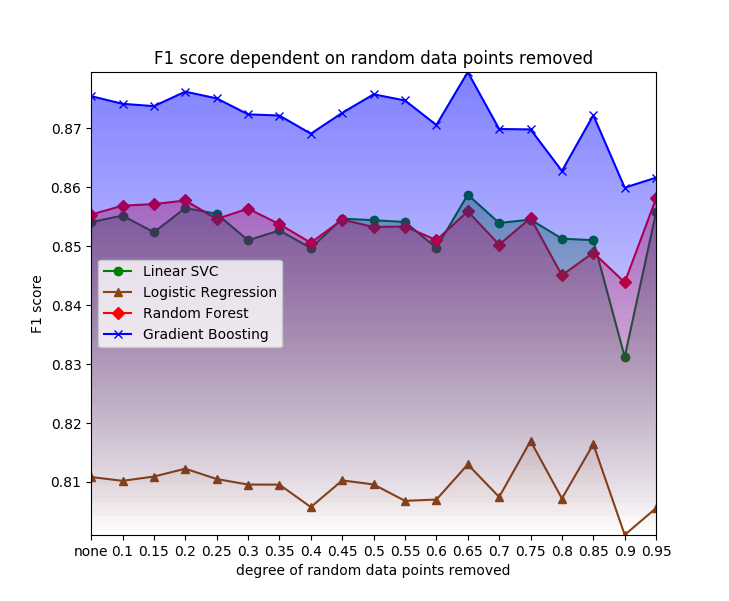
\includegraphics[width=0.49\textwidth]{figures/outliers/randomly_removed_points_all_algos_blur_bright}
	\caption{Binary classification on target income based on a dataset with different degrees of outliers removed (= variance loss) vs. the same degree of data randomly deleted.}
	\label{fig:results_outliers_removed}
\end{figure*}





\subsection{Anonymization on Outliers removed}
\label{ssect:anon_outliers_removed}

\begin{figure*}[!h]
	\centering
	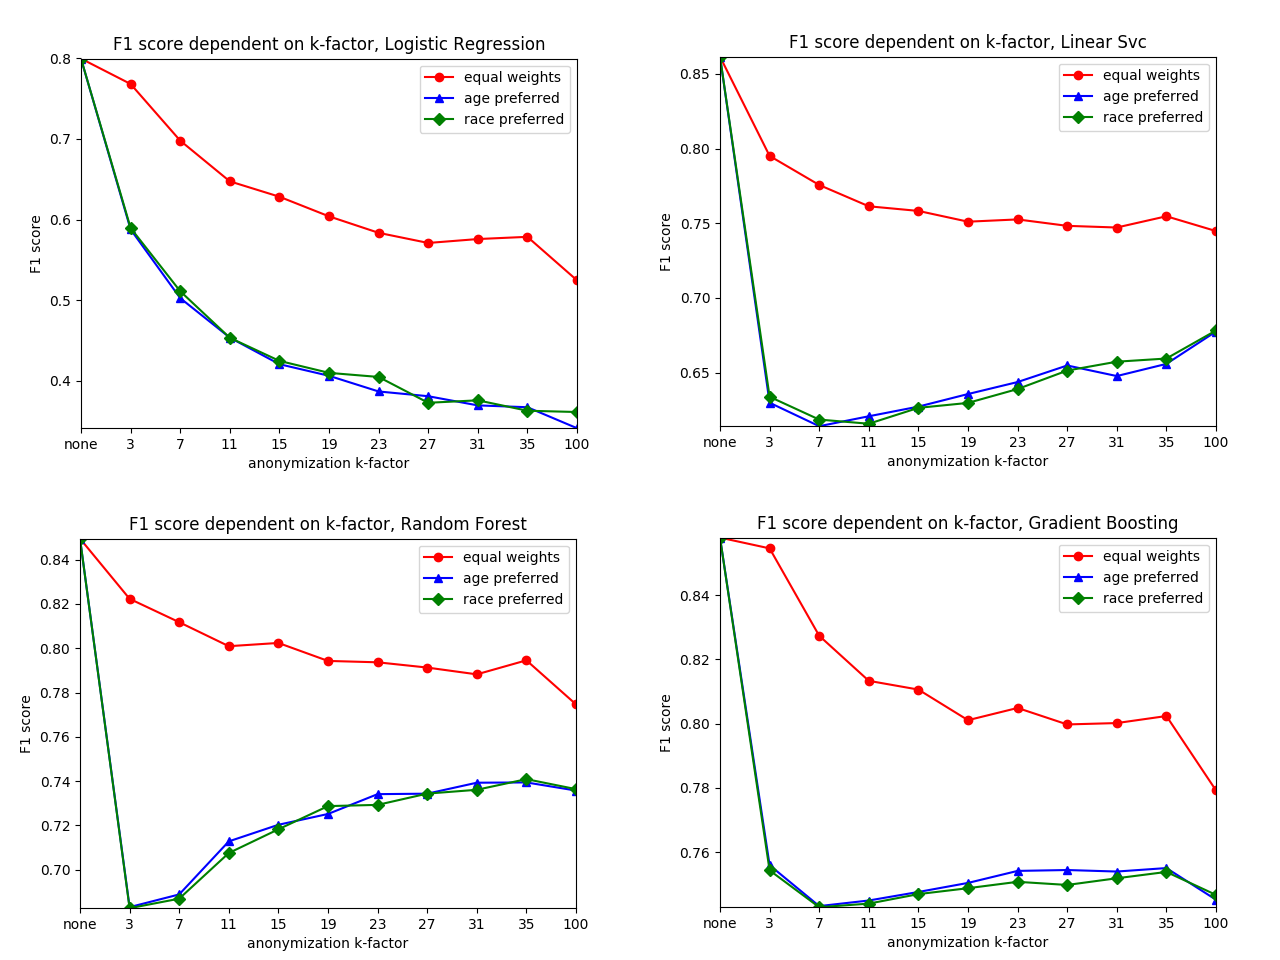
\includegraphics[width=1\textwidth]{figures/anon_outliers/anon_outliers_marital_combined}
	\caption{Multi-class classification on target marital status based on a dataset with 30\% outliers removed AND different degrees of k-anonymization.}
	\label{fig:results_anonymization_outliers_marital_status}
\end{figure*}





% ==================================
%			OPEN PROBLEMS
% ==================================
\section{Open problems Future challenges}
\label{sect:op_fc}

% \begin{itemize}
%	\item \textbf{Explain the unexpected behavior} for the datasets perturbed by selectively deleting rows containing the TOP 3 negatively contributing attribute values.
	
%	\item \textbf{Find a natural dataset} which already contains a graph structure emerged in the real-world rather than a graph generator. We assume that for many modern applications the experiments conducted in this work would be highly relevant to social network analysis and anonymization, and we are planning to conduct such a research effort in a sequel to this investigation.
	
%	\item \textbf{Consider the structural information loss} on a suitable real-world graph and re-apply our methodology to that data-structure. Once realistic results have been obtained, the effects of the same algorithm on artificially generated graphs might be examined, offering another perspective on the information content / structure introduced into datasets by different types of such generators.
	
%	\item \textbf{Analyze the exact influence} different kinds of information loss due to anonymization / perturbation have on the different algorithms. In this work, we have only chosen a series of classifiers to demonstrate our approach. However, other classes of machine learning algorithms might yield interesting results as well, and we are motivated to conduct such future research ourselves.
	
%	\item \textbf{Interactive machine learning}. We have, amongst other settings, experimented with different weight vectors in our approach regarding anonymization. However, such parameters do not easily lend themselves to be produced by an algorithm, since minimizing an artificial metric of information loss  does not produce safe datasets in itself. Moreover, data utility is highly dependent on the specific area of application; therefore choosing parameters with regard to the particular demographic and cultural clinical environment is best done by a human agent. The problem of (k-)anonymization thus represents a natural application domain for interactive Machine Learning (iML) with a human-in-the-loop \cite{Holzinger:2016:iML}, \cite{Kieseberg:2016:Doctor-in-the-Loop}, \cite{iMLExperiment}. The authors will strive to design and implement such experiments in the future.
% \end{itemize}


% ==================================
%			CONCLUSION
% ==================================
\section{Conclusion}
\label{sect:conclusion}

% This paper examined the question of how different ways of perturbing or anonymizing knowledge bases would influence the results of machine learning algorithms applied to those datasets. We have seen that newly introduced regulations (inside the European Union) as well as data privacy concerns of database owners naturally lead to the challenge of minimizing the cost / efficiency impact of those requirements not only on the technical, but also the machine learning infrastructure of affected businesses and organizations. Consequently, we conducted a series of experiments to simulate the decline in the F1 score of several classification algorithms on an established dataset. Our results show that selective deletion of valuable data items is less destructive than general anonymization, so that complying with regulations concerning the "right to be forgotten" is still preferable to taking preemptive steps to de-identify personal information in databases. Our results are highly selective however and should be corroborated by applying a wider spectrum of algorithms to larger, more diverse datasets.


\bibliographystyle{plain}
\bibliography{references}

\end{document}


% \begin {comment}
% \section{Glossary and Key Terms}
% NOTE: this section may not to be used for a conference
% \textbf{Note: This is only for use when producing a Springer LNCS SOTA State-of-the-Art-Analysis paper}
% \\[0,2cm]
% \emph{SaNGreeA} is the abbreviation for Social Network Greedy Anonymization, which describes an anonymization algorithm which takes into account information loss as well as structural loss (from anonymizing the neighborhood of a network node). It is said to be greedy as it uses greedy clustering under the hood in order to avoid having to sift through an exponential solution space to find an optimum.
% \end{comment}
